\chapter{Results}
\label{ch:results}

This chapter reports the results in the order Section~\ref{sec:method-analyses} introduced the analyses. Interpretation is kept for Chapter~\ref{ch:discussion}. Every statistic in this chapter is taken from the analysis result files, and the tables are built from the same files. Each rate is set beside the random-pairing null for its own subset, built by re-pairing image readings and prompts at random \nullShuffles{} times under seed \nullSeed{}, and each interval is a 95\% clustered bootstrap over prompt groups with \DiffDraws{} draws.

\section{Overall agreement}
\label{sec:results-overall}

Table~\ref{tab:headline} is the main table. It holds the four measures for the \nEmotional{} emotional prompts, and Figure~\ref{fig:zgroup} plots each of those cells as a distance from its null, in units of the null's standard deviation. Every rung of the ladder sits above chance. On valence sign the rate is \FullEmoSignObs{} where random re-pairing gives \FullEmoSignNull{} ($z$ = \FullEmoSignZ{}, 95\% confidence interval (CI) \FullEmoSignCi{}). Its denominator is \FullEmoNSign{} of the \FullEmoN{}, because a prompt whose top family is surprise has no valence sign. Family agreement comes to \FullEmoFamObs{} against \FullEmoFamNull{} ($z$ = \FullEmoFamZ{}, CI \FullEmoFamCi{}) and top-3 soft overlap to \FullEmoOvlpObs{} against \FullEmoOvlpNull{} ($z$ = \FullEmoOvlpZ{}). Valence--arousal similarity is \FullEmoVaObs{} against \FullEmoVaNull{} ($z$ = \FullEmoVaZ{}). So the loosest measure gives the largest $z$ of the four, and the smallest gap in points between observed and null. Because of the floor in Equation~\ref{eq:va}, random pairs already score high on this measure and the null barely varies, so a few points above it come to many multiples of the null's spread.

% GENERATED by emoviz/export_tex.py — do not edit
\begin{table}[htbp]
\centering
\small
\caption{Agreement between the prompt reader and the image reader on the 1,012 analysed records, by prompt group and image class, against the random-pairing null (300 re-pairings, seed 7). CI: clustered bootstrap over prompt groups (10,000 draws). n/a: degenerate null (every prompt in the subset shares one label, so permutation cannot change the score).}
\label{tab:headline}
\begin{tabular}{lrrrl}
\toprule
Subset / measure & Observed & Null & $z$ & 95\% CI \\
\midrule
\textbf{Emotional prompts} ($n$=607; sign $n$=530) &  &  &  &  \\
Valence--arousal similarity & 83.8\% & 77.3\% & +12.2 & [82.0, 85.5] \\
Valence-sign agreement & 64.0\% & 45.6\% & +11.1 & [58.6, 68.8] \\
Family agreement & 53.0\% & 38.8\% & +10.3 & [47.3, 58.7] \\
Top-3 soft overlap & 50.6\% & 39.4\% & +11.6 & [46.5, 54.7] \\
\midrule
\textbf{\quad face-classified} ($n$=402; sign $n$=360) &  &  &  &  \\
Valence--arousal similarity & 84.2\% & 76.4\% & +11.2 & [82.3, 86.1] \\
Valence-sign agreement & 73.9\% & 53.5\% & +10.4 & [68.3, 79.2] \\
Family agreement & 61.9\% & 45.8\% & +10.3 & [55.8, 68.0] \\
Top-3 soft overlap & 53.4\% & 40.4\% & +11.6 & [49.2, 57.7] \\
\midrule
\textbf{\quad scene-classified} ($n$=205; sign $n$=170) &  &  &  &  \\
Valence--arousal similarity & 82.9\% & 79.1\% & +6.0 & [80.4, 85.2] \\
Valence-sign agreement & 42.9\% & 29.6\% & +5.8 & [33.1, 51.1] \\
Family agreement & 35.6\% & 26.2\% & +4.4 & [26.4, 44.1] \\
Top-3 soft overlap & 44.9\% & 38.1\% & +4.9 & [38.7, 51.0] \\
\midrule
\textbf{Neutral-labelled prompts} ($n$=405; sign $n$=0) &  &  &  &  \\
Valence--arousal similarity & 76.6\% & 76.6\% & +0.3 & [75.6, 77.6] \\
Valence-sign agreement & 0.0\% & 0.0\% & n/a & degenerate \\
Family agreement & 28.6\% & 28.6\% & n/a & degenerate \\
Top-3 soft overlap & 31.6\% & 31.6\% & +0.0 & -- \\
\bottomrule
\end{tabular}
\end{table}


\begin{figure}[htbp]
\centering
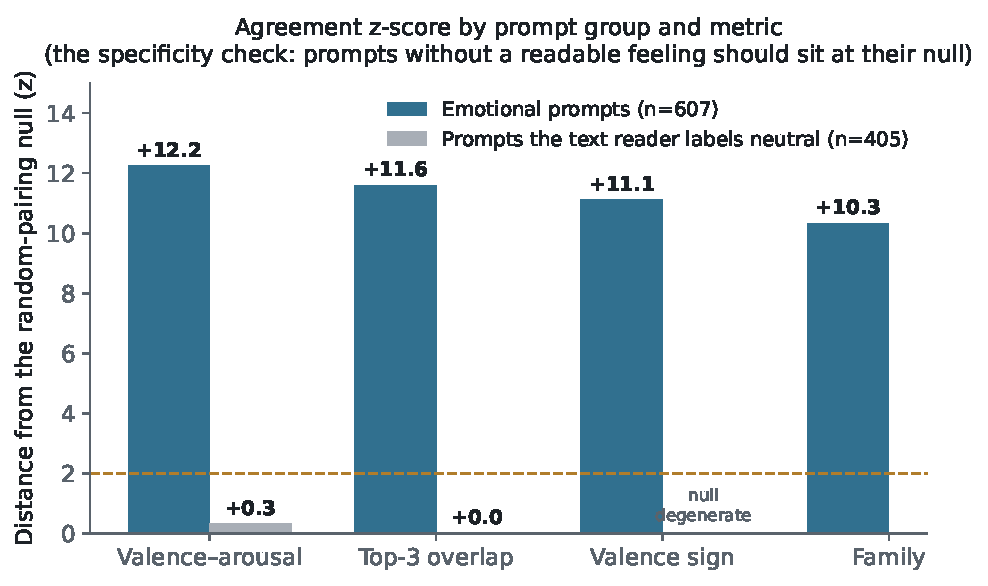
\includegraphics[width=0.9\textwidth]{fig3_z_by_prompt_group}
\caption{Distance from the random-pairing null, in standard deviations of that null ($z$), by prompt group and by measure. The neutral-labelled group has a degenerate null for valence sign and for family, so those two cells are left empty.}
\label{fig:zgroup}
\end{figure}

\section{Face-classified versus scene-classified drawings}
\label{sec:results-face-scene}

Figure~\ref{fig:facescene} and Table~\ref{tab:difference} divide the same \nEmotional{} prompts by the class the describer's answers assign to the drawing. Faces are the larger class, with \FullFaceN{} records. There valence-sign agreement reaches \FullFaceSignObs{} where the null is \FullFaceSignNull{} ($z$ = \FullFaceSignZ{}, CI \FullFaceSignCi{}), and family agreement reaches \FullFaceFamObs{} where the null is \FullFaceFamNull{} ($z$ = \FullFaceFamZ{}). The \FullSceneN{} scene-classified records come out lower on both rungs, at \FullSceneSignObs{} on valence sign (null \FullSceneSignNull{}, $z$ = \FullSceneSignZ{}, CI \FullSceneSignCi{}) and \FullSceneFamObs{} on family (null \FullSceneFamNull{}, $z$ = \FullSceneFamZ{}). In this table both classes clear their nulls. The scene row comes up again in Section~\ref{sec:results-ablation}.

Each class has a null of its own. For that reason the contrast is stated as a difference in percentage points and tested with the clustered permutation procedure from Section~\ref{sec:method-inference}, which gives face minus scene as \DiffSignPp{} for valence sign (clustered interval \DiffSignCi{}) and \DiffFamPp{} for family (interval \DiffFamCi{}). The permutation test returns $p$ = \DiffSignP{} for valence sign and $p$ = \DiffFamP{} for family, the smallest value it can report with the number of permutations run. Valence--arousal similarity hardly moves between the classes (\FullFaceVaObs{} for faces, \FullSceneVaObs{} for scenes), so the gap between them sits in the two categorical rungs.

\begin{figure}[htbp]
\centering
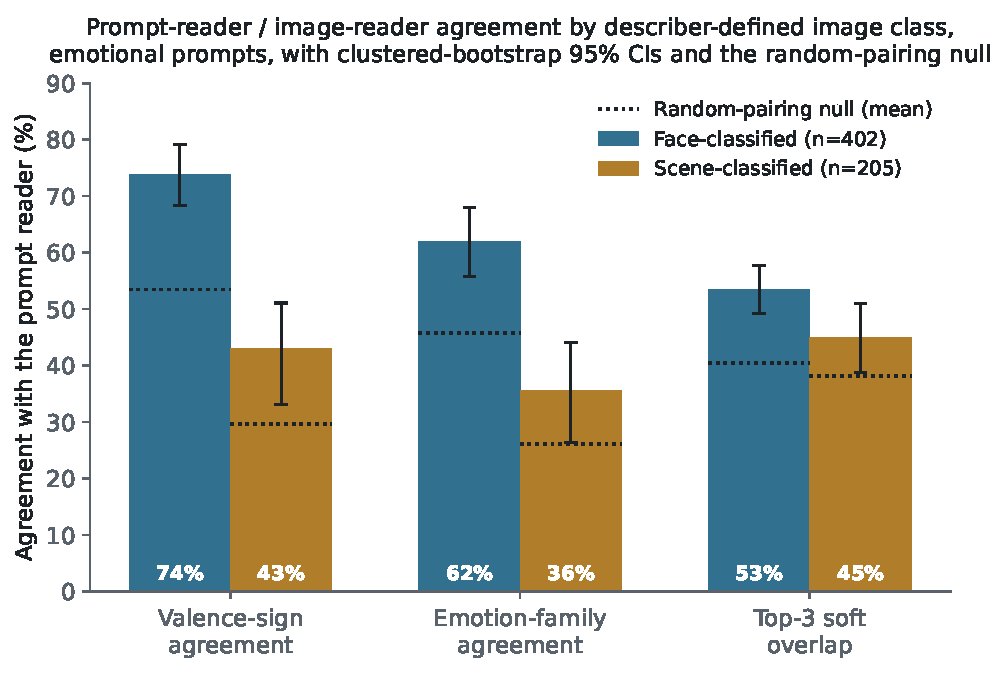
\includegraphics[width=\textwidth]{fig1_face_vs_scene}
\caption{Agreement of the image reader with the prompt reader on the emotional prompts, split by the describer-defined class of the drawing. Error bars are clustered-bootstrap 95\% intervals. The dotted line in each cell is that cell's random-pairing null.}
\label{fig:facescene}
\end{figure}

% GENERATED by emoviz/export_tex.py — do not edit
\begin{table}[htbp]
\centering
\footnotesize
\caption{Face-classified versus scene-classified drawings on the emotional prompts: agreement with 95\% clustered-bootstrap CIs, the difference with its CI, and the clustered permutation p (10,000 draws; significance.py).}
\label{tab:difference}
\begin{tabular}{lllll}
\toprule
Measure & Face ($n$=402) & Scene ($n$=205) & Difference (pp) & Perm.\ $p$ \\
\midrule
Valence-sign agreement & 73.9\% [68.3, 79.2] & 42.9\% [33.1, 51.1] & +30.9~pp [+22.6, +40.6] & 0.0001 \\
Family agreement & 61.9\% [55.8, 68.0] & 35.6\% [26.4, 44.1] & +26.3~pp [+18.4, +35.3] & 0.0001 \\
\bottomrule
\end{tabular}
\end{table}


\section{Distinct prompts and the multiple-comparison correction}
\label{sec:results-robustness}

Because \nRepeats{} records repeat an earlier prompt, Table~\ref{tab:distinct} re-runs the main table with only each prompt's first occurrence kept. That leaves \nDistinct{} records, \nDistinctEmo{} of them emotional. The overall and the face results hold: the \DistFaceN{} face-classified records among the distinct prompts give \DistFaceSignObs{} on valence sign ($z$ = \DistFaceSignZ{}) and \DistFaceFamObs{} on family ($z$ = \DistFaceFamZ{}). The scene row loses a good part of its margin. For the \DistSceneN{} scene-classified records among them, valence sign drops to \DistSceneSignObs{} ($z$ = \DistSceneSignZ{}) and family to \DistSceneFamObs{} ($z$ = \DistSceneFamZ{}).

Table~\ref{tab:holm} runs Holm--Bonferroni over all \HolmM{} of the $z$-scores that are not degenerate. \HolmSurvive{} pass at the family-wise 0.05 level and \HolmFail{} fail. The survivors include the full-sample cells of the emotional subset and of both image classes, and the distinct-prompt cells of the emotional subset and of the face class, so every cell reported so far survives except one. Most of the failures were expected to sit at chance anyway: the neutral-labelled control in both blocks, and the valence--arousal and overlap cells of the two single-valence subsets. The one failure among the reported cells is the scene family cell of the distinct-prompt block at $z$ = \DistSceneFamZ{}. It was expected to be informative, and is treated as suggestive only.

% GENERATED by emoviz/export_tex.py — do not edit
\begin{table}[htbp]
\centering
\small
\caption{The same analysis on the 763 distinct prompts only (first occurrence of each prompt text kept), a check against pseudo-replication from the 249 repeated prompts.}
\label{tab:distinct}
\begin{tabular}{lrrrl}
\toprule
Subset / measure & Observed & Null & $z$ & 95\% CI \\
\midrule
\textbf{Emotional prompts} ($n$=452; sign $n$=394) &  &  &  &  \\
Valence--arousal similarity & 83.0\% & 76.5\% & +10.6 & [81.5, 84.4] \\
Valence-sign agreement & 62.2\% & 44.4\% & +9.9 & [57.2, 67.0] \\
Family agreement & 51.3\% & 37.2\% & +9.3 & [46.7, 56.0] \\
Top-3 soft overlap & 48.9\% & 37.7\% & +10.8 & [45.9, 51.9] \\
\midrule
\textbf{\quad face-classified} ($n$=319; sign $n$=284) &  &  &  &  \\
Valence--arousal similarity & 83.5\% & 75.5\% & +9.7 & [81.7, 85.2] \\
Valence-sign agreement & 71.8\% & 51.0\% & +8.4 & [66.4, 77.0] \\
Family agreement & 59.9\% & 43.0\% & +8.1 & [54.2, 65.2] \\
Top-3 soft overlap & 51.8\% & 38.4\% & +9.7 & [48.1, 55.4] \\
\midrule
\textbf{\quad scene-classified} ($n$=133; sign $n$=110) &  &  &  &  \\
Valence--arousal similarity & 81.8\% & 78.9\% & +3.6 & [79.5, 83.8] \\
Valence-sign agreement & 37.3\% & 27.1\% & +3.5 & [28.1, 46.2] \\
Family agreement & 30.8\% & 24.1\% & +2.6 & [23.3, 38.4] \\
Top-3 soft overlap & 41.7\% & 36.7\% & +3.1 & [36.9, 46.5] \\
\midrule
\textbf{Neutral-labelled prompts} ($n$=311; sign $n$=0) &  &  &  &  \\
Valence--arousal similarity & 76.6\% & 76.4\% & +1.1 & -- \\
Valence-sign agreement & 0.0\% & 0.0\% & n/a & degenerate \\
Family agreement & 27.7\% & 27.7\% & n/a & degenerate \\
Top-3 soft overlap & 31.4\% & 31.1\% & +0.8 & -- \\
\bottomrule
\end{tabular}
\end{table}

% GENERATED by emoviz/export_tex.py — do not edit
\begin{table}[htbp]
\centering
\footnotesize
\caption{Multiple-comparison control over the 36 non-degenerate $z$-scores the analysis prints (12 degenerate ones excluded). Two-sided $p$ by the normal approximation; Holm--Bonferroni at family-wise 0.05: 26 survive, 10 do not.}
\label{tab:holm}
\begin{tabular}{lp{0.78\textwidth}}
\toprule
Outcome & Tests \\
\midrule
Do not survive & DISTINCT negative prompts overlap z+2.7; DISTINCT scene images family z+2.6; FULL positive prompts overlap z+2.3; FULL negative prompts va z+2.1; DISTINCT positive prompts overlap z+1.9; DISTINCT negative prompts va z+1.6; DISTINCT non-emotional va z+1.1; DISTINCT non-emotional overlap z+0.8; FULL non-emotional va z+0.3; FULL non-emotional overlap z+0.0 \\
Survive & the remaining 26, including every headline (emotional, face and scene on all four measures; distinct-prompt emotional and face) \\
\bottomrule
\end{tabular}
\end{table}


\section{Specificity check: prompts the prompt reader labels neutral}
\label{sec:results-control}

The specificity check uses the \CtrlN{} prompts that the prompt reader labelled neutral. Only one measure can move here. Valence sign has a numerator and a denominator of zero on this subset, and the family rate is exactly its null, \CtrlFamObs{}, because every prompt has the same label and re-pairing the drawings cannot change how often the two labels coincide. Valence--arousal similarity does have a live null, and the observed value sits on it: \CtrlVaObs{} against \CtrlVaNull{}, with $z$ = \CtrlVaZ{} at record level and \CtrlVaZClustered{} when the null is clustered on prompt groups.

Table~\ref{tab:control} reports the control audit. \CtrlFlagged{} of the \CtrlN{} (\CtrlFlaggedPct{}) contain at least one word from a fixed lexicon of \CtrlLexicon{} everyday affect words, the commonest being \CtrlTopWords{}, and a further \CtrlNameOnly{} consist of nothing but the redaction placeholder. Removing them leaves a cleaned control of \CtrlCleanN{} records. On those the value is \CtrlCleanVaObs{} against \CtrlCleanVaNull{} ($z$ = \CtrlCleanVaZ{}), the same as before. The null's standard deviation here is only \CtrlVaSd{}, because the prompt-side points hardly vary between neutral prompts, so observed and expected were always going to land close together. The check passes, and weakly, for that reason.

% GENERATED by emoviz/export_tex.py — do not edit
\begin{table}[htbp]
\centering
\small
\caption{The specificity check on the prompts the text reader labels neutral. Only valence--arousal similarity is informative there (sign and family are degenerate: every prompt shares the neutral label). Cleaned control = minus the 2 records reduced to `[name]' and the 68 containing one of 66 plain affect words.}
\label{tab:control}
\begin{tabular}{lrrrrr}
\toprule
Control set & $n$ & VA observed & VA null & $z$ (record null) & $z$ (clustered null) \\
\midrule
All neutral-labelled prompts & 405 & 76.6\% & 76.5\% & +0.5 & -0.1 \\
Cleaned control & 335 & 76.6\% & 76.6\% & +0.0 & -0.6 \\
\bottomrule
\end{tabular}
\end{table}


\section{Two image readers, like for like}
\label{sec:results-method}

Figure~\ref{fig:method} and Table~\ref{tab:method} score the two image readers under identical conditions: one prompt reader, the same \McN{} emotional records, the four measures and one set of random re-pairings. On family agreement describe-then-extract reaches \McDeFam{} and direct CLIP \McClipFam{}. The difference of \McDiffFamPp{} has a clustered interval of \McDiffFamCi{}, the cluster sign-flip test puts $p$ at \McClusterFamP{}, and the exact McNemar test, which takes every record as independent and so errs on the optimistic side, gives $p$ = \McMcNemarFamP{}. Valence sign goes the same way, \McDeSign{} against \McClipSign{} (\McDiffSignPp{}, CI \McDiffSignCi{}), as do overlap (\McDeOvlp{} against \McClipOvlp{}) and valence--arousal similarity (\McDeVa{} against \McClipVa{}). Counting records, \McFamB{} of the \McN{} are agreed on by describe-then-extract alone, \McFamC{} by direct CLIP alone, \McFamBoth{} by both readers and \McFamNeither{} by neither.

Two numbers in the table need a note. Direct CLIP's family $z$ is \McClipFamZ{}, above the \McDeFamZ{} of describe-then-extract, even though its rate is far lower. The reason is that its null sits lower and varies less. Direct CLIP returns neutral for \McClipNeutral{} of the \McN{} images, and an image read as neutral cannot agree by family with any emotional prompt the re-pairing hands it, so chance agreement is rare for it too. A $z$ measures a reader's distance from its own chance level, so the comparison between the readers rests on the paired tests on the rates above. The second number is the two image readers' own agreement, only \McReaderAgree{} on top-1 family. Table~\ref{tab:methodvone} is the first build's version of this comparison, run on \McVOneN{} records with the entailment model on the prompt side too and an earlier overlap formula, so its figures are not comparable with those of the main analysis. It is kept as history only and none of its figures is quoted.

\begin{figure}[htbp]
\centering
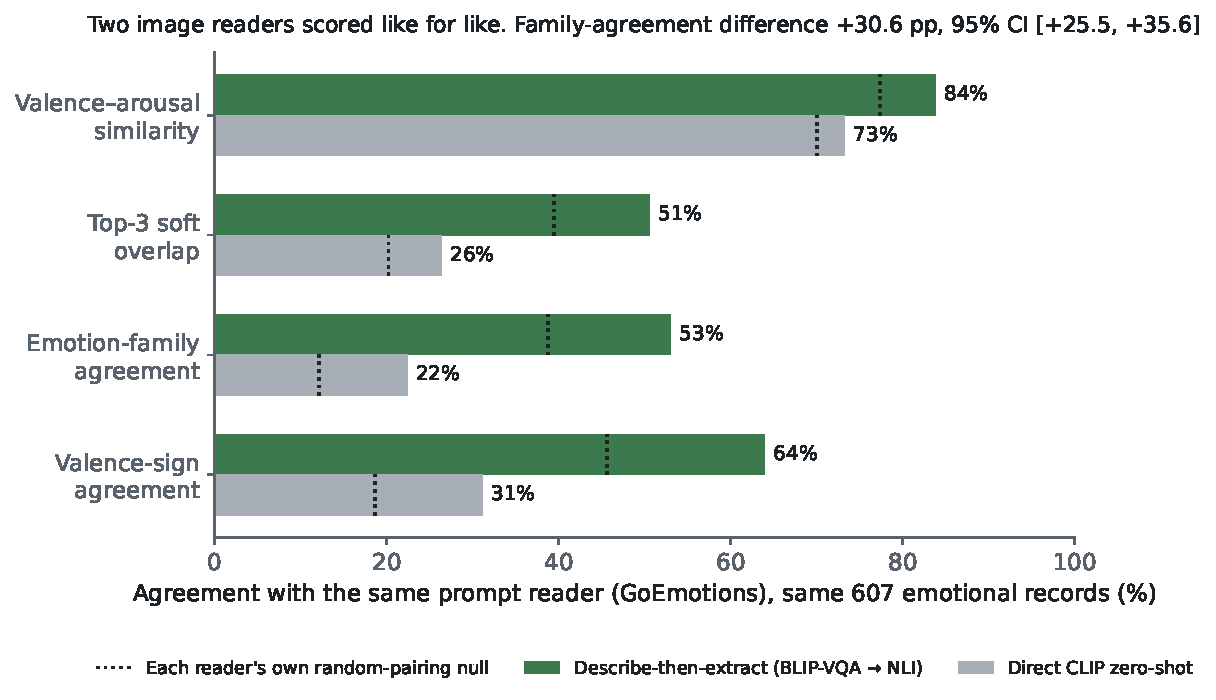
\includegraphics[width=\textwidth]{fig2_method_comparison}
\caption{The two image readers scored against one prompt reader on the same \McN{} emotional records. The dotted mark in each cell is that reader's own random-pairing null.}
\label{fig:method}
\end{figure}

{\setlength{\tabcolsep}{2.5pt}% GENERATED by emoviz/export_tex.py — do not edit
\begin{table}[htbp]
\centering
\scriptsize
\caption{Two image readers scored like for like against the same prompt reader (GoEmotions) on the same 607 emotional records with the same measures and the same 300 re-pairings. $b$ = records only describe-then-extract agrees on; $c$ = records only direct CLIP agrees on. The exact McNemar $p$ treats records as independent and is optimistic ($3.4\times10^{-35}$ for family); the cluster sign-flip randomisation (20,000 draws) respects prompt groups.}
\label{tab:method}
\begin{tabular}{lrrrrrr}
\toprule
Measure & Describe→extract & null & $z$ & Direct CLIP & null & $z$ \\
\midrule
Valence--arousal similarity & 83.8\% & 77.3\% & +12.2 & 73.3\% & 70.1\% & +10.2 \\
Valence-sign agreement & 64.0\% & 45.6\% & +11.1 & 31.1\% & 18.6\% & +9.9 \\
Family agreement & 53.0\% & 38.8\% & +10.3 & 22.4\% & 12.2\% & +11.1 \\
Top-3 soft overlap & 50.6\% & 39.4\% & +11.6 & 26.4\% & 20.2\% & +11.2 \\
\midrule
Paired family test & $b$=218, $c$=32 &  &  & diff +30.6~pp & CI [+25.5, +35.6] & cluster $p<0.001$ \\
Paired valence-sign test & $b$=204, $c$=30 &  &  & diff +32.8~pp & CI [+27.4, +38.2] & cluster $p<0.001$ \\
\bottomrule
\end{tabular}
\end{table}
}
% GENERATED by emoviz/export_tex.py — do not edit
\begin{table}[htbp]
\centering
\small
\caption{The earlier (v1) comparison as published in the build log: prompt side read by BART-MNLI, the 608 records of the v1 lexicon rule, and a different overlap formula. Kept as a record; not comparable with Table~\ref{tab:headline}.}
\label{tab:methodvone}
\begin{tabular}{lrr}
\toprule
Measure & Describe→extract & Direct CLIP \\
\midrule
Family agreement & 49.3\% & 25.3\% \\
Top-3 soft overlap & 48.6\% & 22.8\% \\
Valence--arousal similarity & 83.7\% & 74.2\% \\
\bottomrule
\end{tabular}
\end{table}


\section{Consistency across repeated prompts}
\label{sec:results-consistency}

Repeated prompts form \nGroups{} groups, which cover \nGroupRecords{} records. \nPairGroups{} of them are pairs. Figure~\ref{fig:consistency} and Table~\ref{tab:consistency} report how often the drawings in a group get the same reading. Averaged over groups, the share of a group's drawings given its modal family is \ConsFam{}, with a bootstrap interval over groups of \ConsFamCi{}. The permutation null shuffles image families over every analysed record and re-cuts the same groups, and it gives \ConsFamNull{} with a standard deviation of \ConsFamNullSd{}, so $z$ = \ConsFamZ{} and the permutation $p$ is \ConsFamP{}. On valence sign the within-group share is \ConsVal{} against \ConsValNull{} ($z$ = \ConsValZ{}). Groups in which every drawing received one family, the fully consistent ones, number \ConsFull{} of \nGroups{} (\ConsFullPct{}), where \ConsFullNull{} would be expected by chance ($z$ = \ConsFullZ{}). For the \nPairGroups{} pairs the share can only be one half or one, which puts a floor under the mean.

The largest group is the single word ``happy'', drawn \ConsHappyN{} times. Of those drawings the image reader returned joy for \ConsHappyJoy{}, neutral for \ConsHappyNeutral{} and surprise for \ConsHappySurprise{}, and Figure~\ref{fig:happygrid} lays out a selection of them with the reader's family printed under each.

\begin{figure}[htbp]
\centering
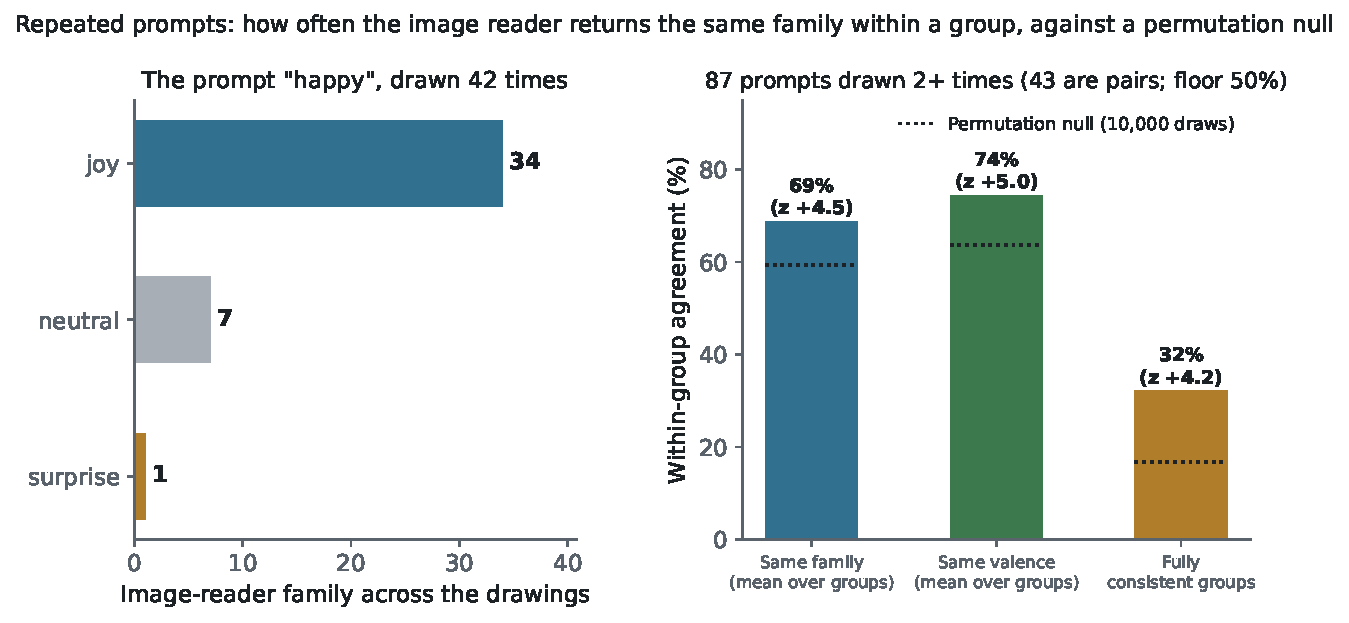
\includegraphics[width=\textwidth]{fig4_consistency}
\caption{Repeated prompts. Left: the image reader's top-1 family over the \ConsHappyN{} drawings of ``happy''. Right: for all \nGroups{} repeated prompts, the share of a group's drawings given its modal family, with the permutation null.}
\label{fig:consistency}
\end{figure}

\begin{figure}[htbp]
\centering
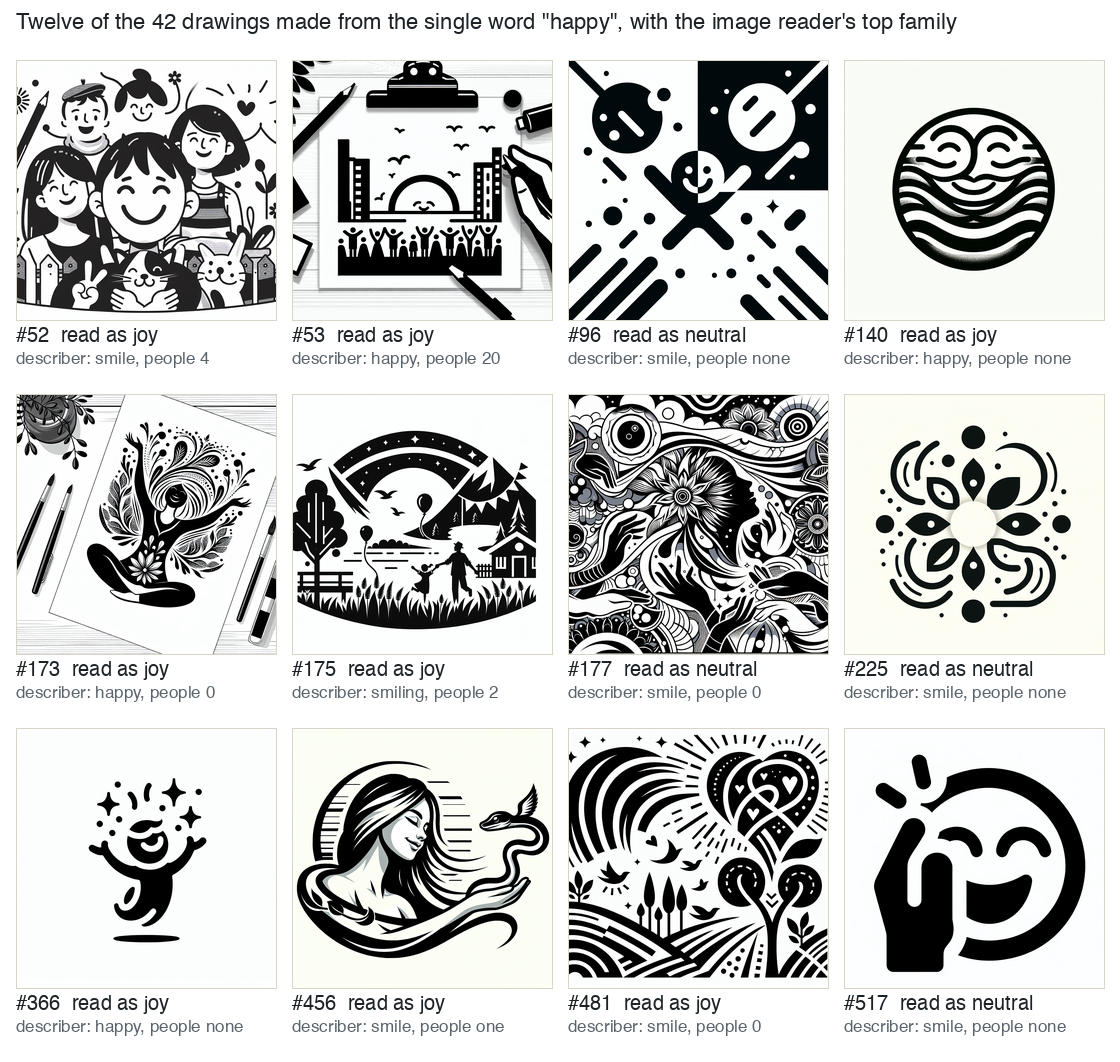
\includegraphics[width=\textwidth]{fig_happy_grid}
\caption{Twelve of the \ConsHappyN{} drawings made from the prompt ``happy'', each with the family the image reader returned for it.}
\label{fig:happygrid}
\end{figure}

% GENERATED by emoviz/export_tex.py — do not edit
\begin{table}[htbp]
\centering
\small
\caption{Within-group agreement of the image reader across the 87 prompts drawn two or more times (336 records; 43 groups are pairs, whose modal agreement cannot fall below 50\%), against a permutation null that shuffles the image readings over all 1,012 analysed records and re-cuts them into the same groups (10,000 draws, seed 7).}
\label{tab:consistency}
\begin{tabular}{lrrrr}
\toprule
Quantity & Observed & Null mean (sd) & $z$ & $p$ \\
\midrule
Same family, mean over groups & 68.8\% & 59.4\% (2.1\%) & +4.5 & $1.0\times10^{-4}$ \\
Same valence, mean over groups & 74.5\% & 63.7\% (2.1\%) & +5.0 & $1.0\times10^{-4}$ \\
Fully consistent groups (of 87) & 28 & 14.5 (3.2) & +4.2 & $2.0\times10^{-4}$ \\
\bottomrule
\end{tabular}
\end{table}


\section{Per-family agreement}
\label{sec:results-families}

Figure~\ref{fig:confusion} and Table~\ref{tab:confusion} tabulate the image reader's family against the prompt reader's for the \nEmotional{} emotional records, and Table~\ref{tab:families} gives the marginals of both readers over all \nAnalysed{} analysed records. Joy dominates the prompt side. It accounts for \RecJoyN{} of the emotional prompts, sadness for \RecSadnessN{} and surprise for \RecSurpriseN{}, while fear (\RecFearN{}), anger (\RecAngerN{}) and disgust (\RecDisgustN{}) are rare. Recall by prompt family is defined per row: of the prompts the prompt reader assigns to a family, the share whose drawing the image reader also assigns to it. Joy has recall \RecJoy{} (CI \RecJoyCi{}) and sadness \RecSadness{} (CI \RecSadnessCi{}); surprise is at \RecSurprise{} (CI \RecSurpriseCi{}), anger at \RecAnger{} on only \RecAngerN{} prompts and fear at \RecFear{} on \RecFearN{}. Disgust never comes back from the image reader. Fear comes back \famImageFear{} times in \nAnalysed{} records.

Table~\ref{tab:kappa} gives Cohen's kappa for family agreement. For the emotional prompts it is \KappaEmo{} (CI \KappaEmoCi{}), the face-classified records give \KappaFace{} and the scene-classified \KappaScene{}, which the Landis--Koch bands call \KappaEmoBand{}, \KappaFaceBand{} and \KappaSceneBand{} in that order. In practice family agreement can be read on three families, joy, sadness and neutral. Anger comes fourth, and it is too rare on the prompt side, as are fear and disgust, for a claim about any one of the three.

\begin{figure}[htbp]
\centering
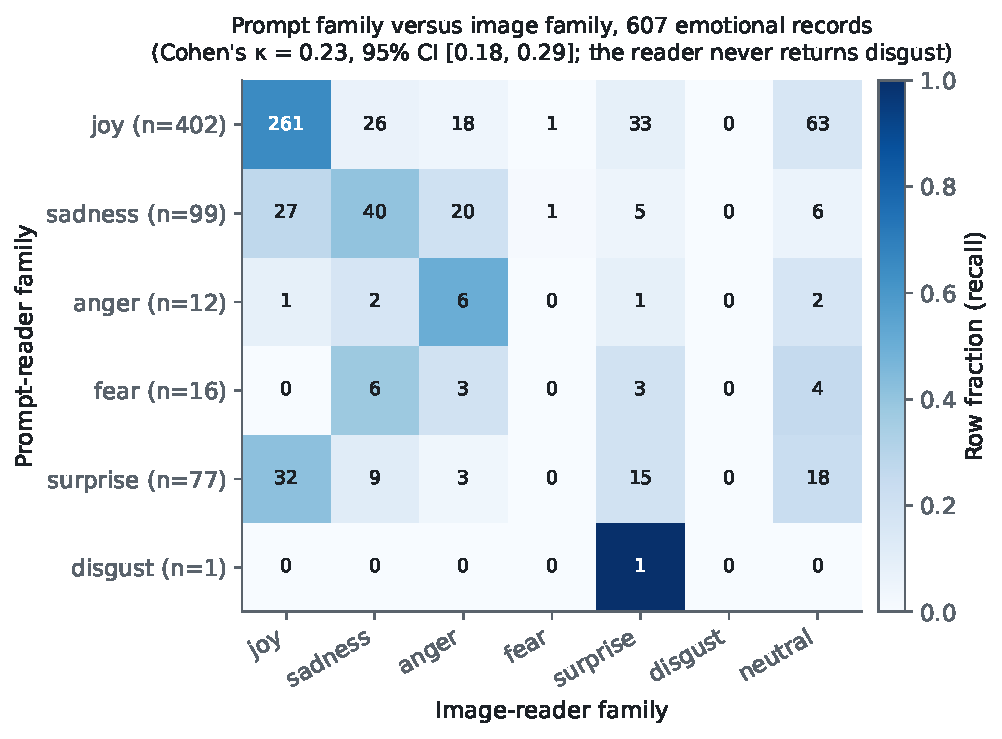
\includegraphics[width=0.85\textwidth]{fig6_confusion}
\caption{Prompt-reader family (rows) crossed with image-reader family (columns) on the \nEmotional{} emotional records. Each cell holds a count, and the shading is the share of the row.}
\label{fig:confusion}
\end{figure}

% GENERATED by emoviz/export_tex.py — do not edit
\begin{table}[htbp]
\centering
\scriptsize
\caption{Prompt-reader family (rows) against image-reader family (columns) on the 607 emotional records. Recall = row diagonal share, with a clustered-bootstrap 95\% CI. Cohen's $\kappa$ = 0.23 [0.18, 0.29]. The image reader never returns disgust and returns fear 4 times in 1,012 records.}
\label{tab:confusion}
\begin{tabular}{lrrrrrrrrl}
\toprule
Prompt \textbackslash{} image & joy & sadness & anger & fear & surprise & disgust & neutral & $n$ & Recall [CI] \\
\midrule
joy & 261 & 26 & 18 & 1 & 33 & 0 & 63 & 402 & 64.9\% [59, 70] \\
sadness & 27 & 40 & 20 & 1 & 5 & 0 & 6 & 99 & 40.4\% [31, 51] \\
anger & 1 & 2 & 6 & 0 & 1 & 0 & 2 & 12 & 50.0\% [22, 78] \\
fear & 0 & 6 & 3 & 0 & 3 & 0 & 4 & 16 & 0.0\% [0, 0] \\
surprise & 32 & 9 & 3 & 0 & 15 & 0 & 18 & 77 & 19.5\% [11, 28] \\
disgust & 0 & 0 & 0 & 0 & 1 & 0 & 0 & 1 & 0.0\% [0, 0] \\
\midrule
\textit{image total} & 321 & 83 & 50 & 2 & 58 & 0 & 93 & 607 &  \\
\bottomrule
\end{tabular}
\end{table}

% GENERATED by emoviz/export_tex.py — do not edit
\begin{table}[htbp]
\centering
\small
\caption{Cohen's $\kappa$ for family agreement (7 families), with clustered-bootstrap 95\% CIs and the Landis \& Koch (1977) band. The neutral-labelled subset is degenerate ($\kappa$ = 0 by construction) and is omitted.}
\label{tab:kappa}
\begin{tabular}{lrrll}
\toprule
Subset & $n$ & $\kappa$ & 95\% CI & Band \\
\midrule
emotional & 607 & 0.23 & [0.18, 0.29] & fair \\
face & 402 & 0.30 & [0.23, 0.37] & fair \\
scene & 205 & 0.13 & [0.06, 0.19] & slight \\
all analysed & 1012 & 0.21 & [0.16, 0.25] & fair \\
distinct emotional & 452 & 0.23 & [0.17, 0.29] & fair \\
distinct face & 319 & 0.29 & [0.21, 0.37] & fair \\
distinct scene & 133 & 0.09 & [0.01, 0.17] & slight \\
\bottomrule
\end{tabular}
\end{table}

% GENERATED by emoviz/export_tex.py — do not edit
\begin{table}[htbp]
\centering
\small
\caption{Top-1 family marginals of the two readers over all 1,012 analysed records.}
\label{tab:families}
\begin{tabular}{lrr}
\toprule
Family & Prompt reader & Image reader \\
\midrule
joy & 402 & 461 \\
sadness & 99 & 141 \\
anger & 12 & 89 \\
fear & 16 & 4 \\
surprise & 77 & 108 \\
disgust & 1 & 0 \\
neutral & 405 & 209 \\
\bottomrule
\end{tabular}
\end{table}


\section{The describer}
\label{sec:results-describer}

Table~\ref{tab:describer} tabulates, for all \nAnalysed{} records, the people count the describer gives against whether its expression answer contains an expression word, so the cells separate the records with a person and an expression word from those with only one of the two and those with neither. The expression question never gets a blank. For \DescNoPeopleExpr{} records it names an expression while its own people count says nobody is there. The scene-classified records number \DescSceneN{}, and for \DescScenePeopleZero{} of them the people count is zero, yet an expression word is present in \DescScenePeopleZeroExpr{} of those. Of the \DescScenePeopleZero{} records with no reported person, \DescSceneSmile{} (\DescSceneSmilePct{}) give ``smile'', ``smiling'' or ``happy'' as the expression. Figure~\ref{fig:noperson} shows four such drawings with all five answers. The smile rate is given with both denominators: \DescSmileAll{} over all \nAnalysed{} analysed records, \DescSmileFace{} over the \nFaceAll{} face-classified ones.

Copy rate means the share of records on which the image reader returns the family of the describer's own expression answer. On the strict definition the answer must be an emotion word. That is so for \DescBareStrictN{} records, \DescBareStrictPct{} of the corpus, and for those records the family the image reader returns is the family of the describer's own word \DescCopyStrict{} of the time. The broad definition also counts a facial action, ``smile'' or ``crying'' for instance, and covers \DescBareBroadN{} records. On it the copy rate is \DescCopyBroad{} overall, \DescCopyBroadPeople{} when the describer reports a person and \DescCopyBroadPeopleZero{} when it reports none. With the ``0 people'' token in the description, the reading is pulled towards neutral.

% GENERATED by emoviz/export_tex.py — do not edit
\begin{table}[htbp]
\centering
\small
\caption{The describer's answers on all 1,012 analysed records: people count crossed with whether the facial-expression answer contains an expression word. The face rule is the top-left cell. Of the 421 scene-classified records, 414 report no people and 406 of those still contain an expression word (332 answer smile, smiling or happy).}
\label{tab:describer}
\begin{tabular}{lrr}
\toprule
 & Expression word present & Expression word absent \\
\midrule
People $\geq 1$ & 591 & 7 \\
People $= 0$ & 406 & 8 \\
\bottomrule
\end{tabular}
\end{table}


\begin{figure}[htbp]
\centering
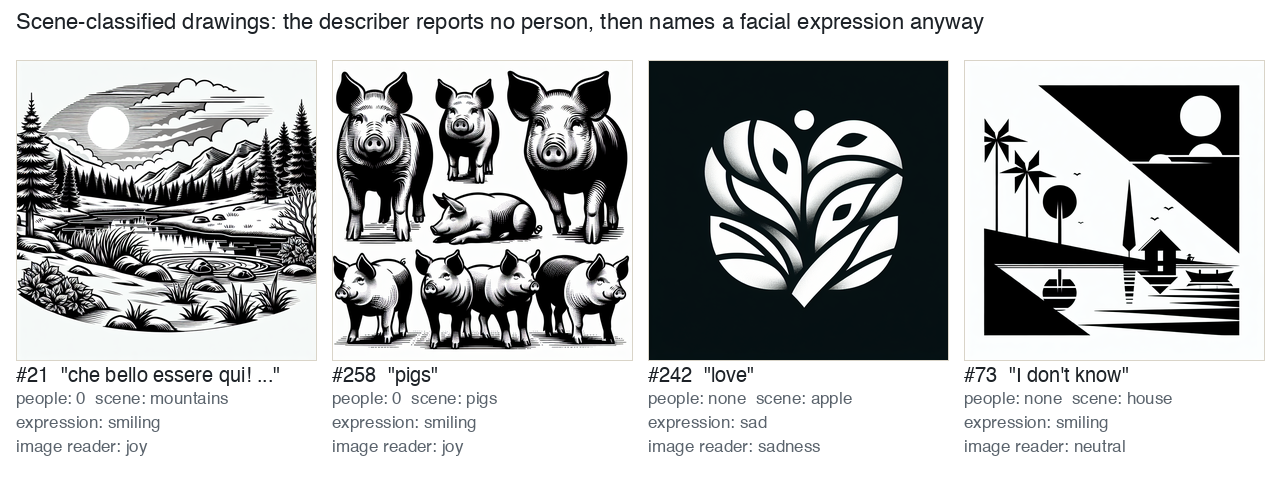
\includegraphics[width=\textwidth]{fig_no_person_expression}
\caption{Four scene-classified drawings for which the describer reported no person and still named a facial expression, each with its five answers as given.}
\label{fig:noperson}
\end{figure}

\section{Error taxonomy}
\label{sec:results-taxonomy}

The taxonomy covers the emotional records where each reader gives its top family a score of at least 0.8 and the two families differ. There are \TaxN{} of them, covering \TaxDistinct{} distinct prompts. The intention was to sample 40, but fewer than that qualified, so every one was examined. Figure~\ref{fig:taxonomy} and Table~\ref{tab:taxonomy} count the primary failure mode, which was assigned by looking at the drawing. The describer is behind \TaxDescriber{} of the \TaxN{}, \TaxA{} of those because a face or an expression it reported is not in the drawing and \TaxB{} because it misread one that is. The image reader accounts for \TaxReader{}, where the description was fair to the drawing and the entailment step still returned another family. \TaxPrompt{} trace to the prompt side, \TaxD{} of them mixed or ambiguous prompts and \TaxF{} a prompt the prompt reader mislabelled, and \TaxGenerator{} to the generator, where the drawing does not depict what the prompt says. Record 137, ``i am excited'', drawn as a screaming face, is one of the \TaxGenerator{} generator cases.

The table shows two patterns. A people count of zero goes with the invented-expression mode, since \TaxPeopleZero{} of the \TaxN{} records have the ``0 people'' tag and most of the \TaxA{} invented-expression records are among them. One mechanism accounts for the joy-to-neutral cell. ``grateful'' and ``calm but tired'' are two of the prompts in it, and both name a low-arousal positive state that none of the seven families has room for, so the describer's answer is ``calm'' or ``smile'' and the image reader returns neutral. The automatic detector for mixed prompts looked for connectives such as ``but'' and ``although''. It caught none of the \TaxD{} mixed prompts, because visitors tend to list feelings with no connective at all, as in ``tired proud happy'', and a detector that looks for a list would do better.

\begin{figure}[htbp]
\centering
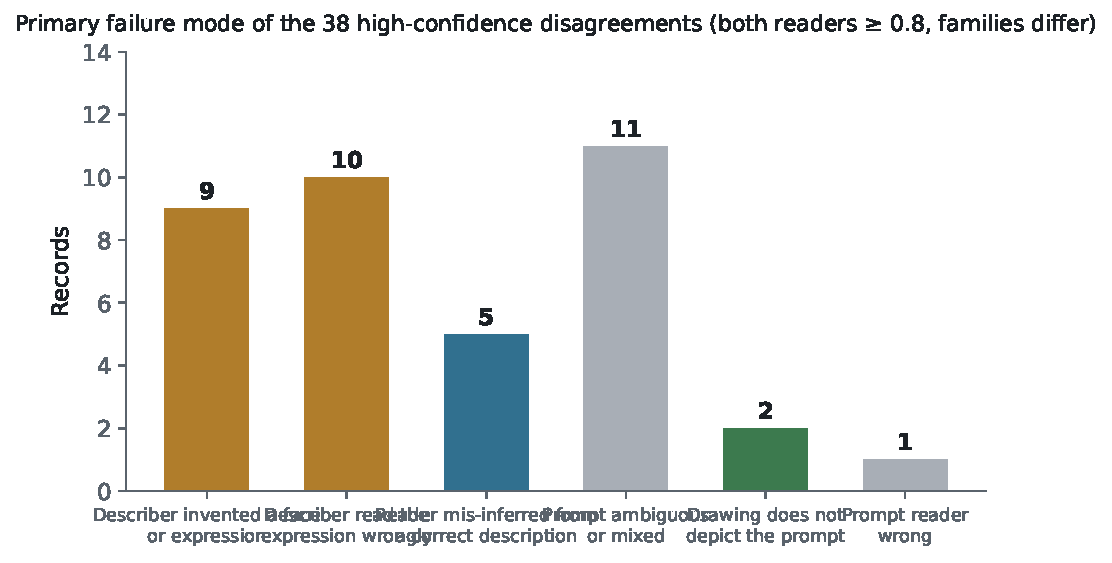
\includegraphics[width=0.95\textwidth]{fig7_error_taxonomy}
\caption{Primary failure mode of the \TaxN{} high-confidence disagreements. Each was assigned by looking at the drawing.}
\label{fig:taxonomy}
\end{figure}

% GENERATED by emoviz/export_tex.py — do not edit
\begin{table}[htbp]
\centering
\small
\caption{Primary failure mode of the 38 high-confidence disagreements (both readers' top-1 score $\geq 0.8$, families differ), assigned from the drawing. Describer faults (a+b) = 19; image reader (c) = 5; prompt side (d+f) = 12; generator (e) = 2.}
\label{tab:taxonomy}
\begin{tabular}{lp{0.55\textwidth}rl}
\toprule
Mode & Description & $n$ & Exemplar ids \\
\midrule
(a) & describer invented a face or expression where none is drawn & 9 & 18, 19, 242 \\
(b) & describer read the expression wrongly & 10 & 39, 192, 202 \\
(c) & reader mis-inferred from a correct description & 5 & 89, 107, 231 \\
(d) & prompt ambiguous or mixed & 11 & 65, 66, 93 \\
(e) & drawing does not depict the prompt & 2 & 137, 771 \\
(f) & prompt reader wrong & 1 & 436 \\
\bottomrule
\end{tabular}
\end{table}


\section{Description-template ablation}
\label{sec:results-ablation}

The template ablation is in Table~\ref{tab:ablation} and Figure~\ref{fig:ablation}, one row per altered description template. Only the entailment stage was re-run. As a control the unmodified template was re-run through the same code path, and the number of records whose top-1 reading changed was \AblControlChanged{}, so the re-run is exact and every difference in the table comes from the template change. The unmodified row reproduces Section~\ref{sec:results-overall}.

Dropping the expression sentence removes most of the agreement. For the emotional prompts, family agreement goes from \FullEmoFamObs{} down to \AblDropExpressionEmoFamObs{}, where the null is \AblDropExpressionEmoFamNull{} ($z$ = \AblDropExpressionEmoFamZ{}), and valence sign from \FullEmoSignObs{} down to \AblDropExpressionEmoSignObs{}, null \AblDropExpressionEmoSignNull{} ($z$ = \AblDropExpressionEmoSignZ{}). The face-classified records alone end at \AblDropExpressionFaceSignObs{} on valence sign. With the expression sentence gone, the image reader's output piles up on two families, surprise on \AblDropExpressionSurprise{} of the \nAnalysed{} records and neutral on \AblDropExpressionNeutral{}. Holding the expression word at ``unclear'' for every record collapses the ladder in the same way, with family agreement at \AblFixedExpressionEmoFamObs{} ($z$ = \AblFixedExpressionEmoFamZ{}). The other clauses matter less. Taking out the action clause, or the posture or scene clause, instead shifts family agreement by between one and three points, to \AblDropActionEmoFamObs{}, \AblDropPostureEmoFamObs{} and \AblDropSceneEmoFamObs{}. Dropping the people count raises the rates and the nulls together, the scene valence-sign cell going to \AblDropPeopleSceneSignObs{} against \AblDropPeopleSceneSignNull{} ($z$ = \AblDropPeopleSceneSignZ{}). Without the ``0 people'' token holding scene readings near neutral, the invented smile reads as joy, and joy is the top family of most emotional prompts.

Under the people-aware template the whole description becomes ``A drawing showing \{scene\}.'' for any record whose people count is zero, and nothing else changes. The face rows cannot change under it. They stay at \AblPeopleAwareFaceSignObs{} and \AblPeopleAwareFaceFamObs{}, identical to the unmodified template by construction, because a face-classified record always has a person reported and so keeps its full description. The scene rows both fall to their nulls, on valence sign \AblPeopleAwareSceneSignObs{} where the null is \AblPeopleAwareSceneSignNull{} ($z$ = \AblPeopleAwareSceneSignZ{}), and on family \AblPeopleAwareSceneFamObs{} where the null is \AblPeopleAwareSceneFamNull{} ($z$ = \AblPeopleAwareSceneFamZ{}). Putting the action and posture clauses back for those records gives the scene cells \AblPeopleAwareNoExpressionSceneSignObs{} on valence sign, null \AblPeopleAwareNoExpressionSceneSignNull{} ($z$ = \AblPeopleAwareNoExpressionSceneSignZ{}), and \AblPeopleAwareNoExpressionSceneFamObs{} on family, null \AblPeopleAwareNoExpressionSceneFamNull{} ($z$ = \AblPeopleAwareNoExpressionSceneFamZ{}). Taken over every emotional prompt, the people-aware template gives \AblPeopleAwareEmoSignObs{} on valence sign ($z$ = \AblPeopleAwareEmoSignZ{}) and \AblPeopleAwareEmoFamObs{} on family ($z$ = \AblPeopleAwareEmoFamZ{}).

\begin{figure}[htbp]
\centering
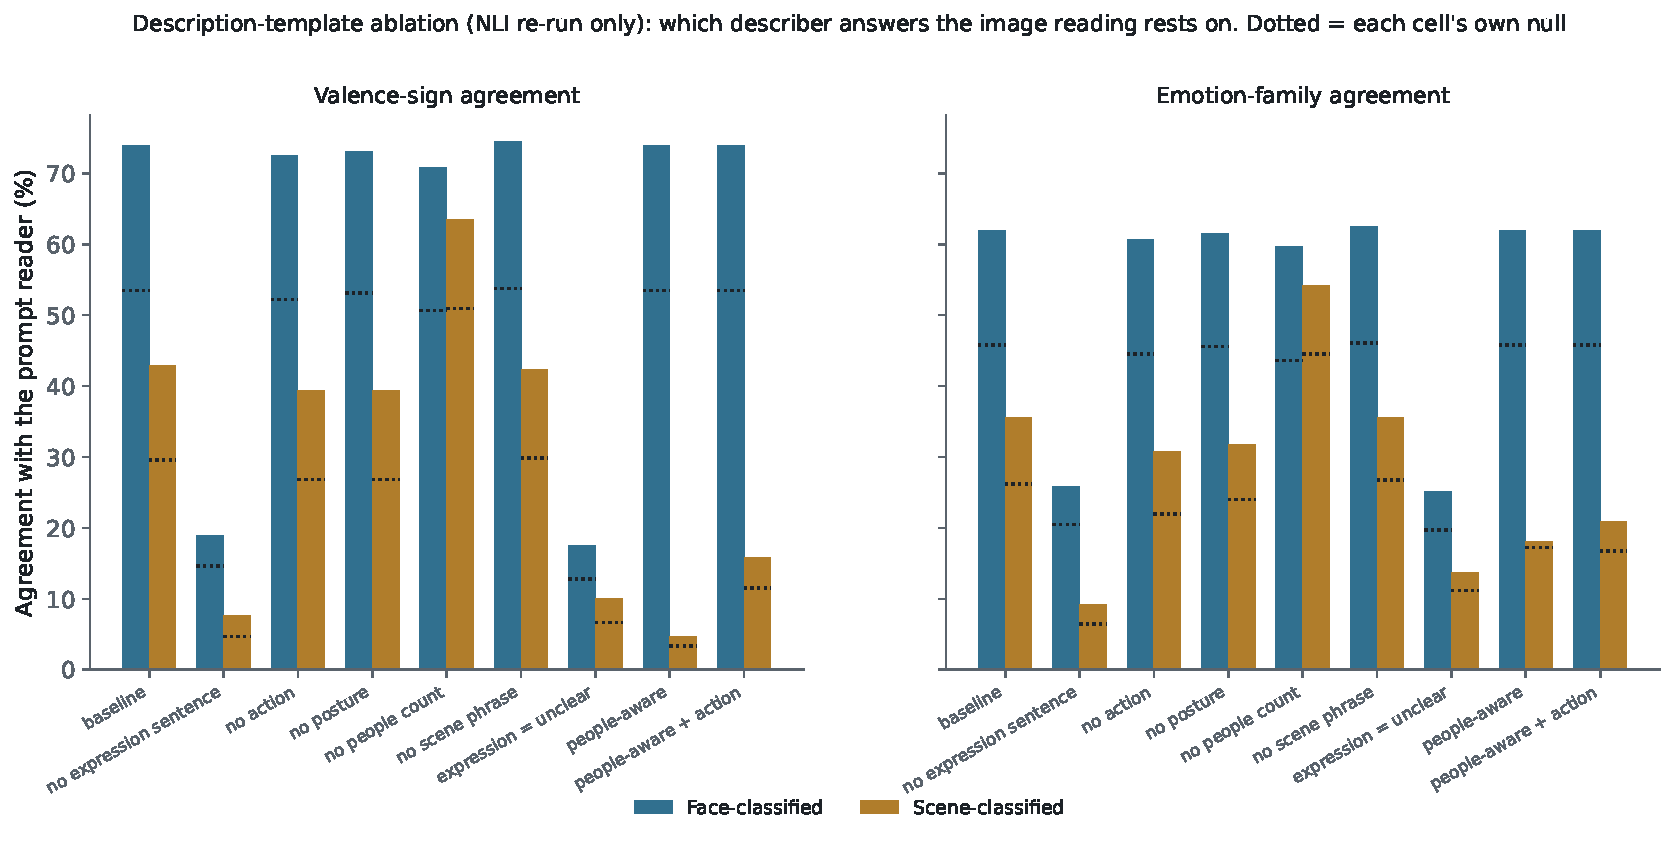
\includegraphics[width=\textwidth]{fig8_ablation}
\caption{Description-template ablation with only the entailment stage re-run. Valence-sign and family agreement by image class under each template. The dotted line in each cell is that cell's random-pairing null.}
\label{fig:ablation}
\end{figure}

% GENERATED by emoviz/export_tex.py — do not edit
\begin{table}[htbp]
\centering
\footnotesize
\caption{Description-template ablation: the NLI stage re-run on descriptions rebuilt from the cached describer answers with one clause removed or fixed; the prompt side and the null procedure unchanged. Valence-sign and family agreement per variant on the emotional prompts and their face/scene halves.}
\label{tab:ablation}
\begin{tabular}{llrrrrrrr}
\toprule
Variant & Subset & $n$ & Sign obs & null & $z$ & Family obs & null & $z$ \\
\midrule
baseline & emotional & 607 & 64.0\% & 45.6\% & +11.1 & 53.0\% & 38.8\% & +10.3 \\
 & face & 402 & 73.9\% & 53.5\% & +10.4 & 61.9\% & 45.8\% & +10.3 \\
 & scene & 205 & 42.9\% & 29.6\% & +5.8 & 35.6\% & 26.2\% & +4.4 \\
\midrule
drop\_expression & emotional & 607 & 15.3\% & 11.4\% & +5.1 & 20.3\% & 16.6\% & +3.8 \\
 & face & 402 & 18.9\% & 14.7\% & +3.8 & 25.9\% & 20.5\% & +3.8 \\
 & scene & 205 & 7.6\% & 4.7\% & +2.7 & 9.3\% & 6.4\% & +2.2 \\
\midrule
drop\_action & emotional & 607 & 61.9\% & 43.9\% & +11.0 & 50.6\% & 36.7\% & +10.3 \\
 & face & 402 & 72.5\% & 52.2\% & +10.4 & 60.7\% & 44.5\% & +10.4 \\
 & scene & 205 & 39.4\% & 26.8\% & +5.6 & 30.7\% & 21.9\% & +4.6 \\
\midrule
drop\_posture & emotional & 607 & 62.3\% & 44.5\% & +10.7 & 51.4\% & 37.9\% & +9.7 \\
 & face & 402 & 73.1\% & 53.1\% & +10.0 & 61.4\% & 45.6\% & +10.1 \\
 & scene & 205 & 39.4\% & 26.8\% & +5.6 & 31.7\% & 24.0\% & +3.6 \\
\midrule
drop\_people & emotional & 607 & 68.5\% & 50.7\% & +10.8 & 57.8\% & 43.7\% & +9.9 \\
 & face & 402 & 70.8\% & 50.7\% & +10.4 & 59.7\% & 43.6\% & +10.3 \\
 & scene & 205 & 63.5\% & 50.9\% & +5.0 & 54.1\% & 44.5\% & +3.8 \\
\midrule
drop\_scene & emotional & 607 & 64.2\% & 46.0\% & +10.7 & 53.4\% & 39.2\% & +9.8 \\
 & face & 402 & 74.4\% & 53.8\% & +10.4 & 62.4\% & 46.1\% & +10.1 \\
 & scene & 205 & 42.4\% & 29.9\% & +5.6 & 35.6\% & 26.8\% & +3.9 \\
\midrule
fixed\_expression & emotional & 607 & 15.1\% & 10.8\% & +5.9 & 21.3\% & 17.5\% & +3.9 \\
 & face & 402 & 17.5\% & 12.8\% & +4.4 & 25.1\% & 19.7\% & +4.0 \\
 & scene & 205 & 10.0\% & 6.6\% & +2.8 & 13.7\% & 11.2\% & +1.5 \\
\midrule
people\_aware & emotional & 607 & 51.7\% & 36.9\% & +10.1 & 47.1\% & 34.5\% & +8.8 \\
 & face & 402 & 73.9\% & 53.5\% & +10.4 & 61.9\% & 45.8\% & +10.3 \\
 & scene & 205 & 4.7\% & 3.4\% & +1.6 & 18.0\% & 17.3\% & +0.6 \\
\midrule
people\_aware\_no\_expression & emotional & 607 & 55.3\% & 39.5\% & +10.5 & 48.1\% & 35.0\% & +9.6 \\
 & face & 402 & 73.9\% & 53.5\% & +10.4 & 61.9\% & 45.8\% & +10.3 \\
 & scene & 205 & 15.9\% & 11.6\% & +2.7 & 21.0\% & 16.8\% & +2.2 \\
\midrule
control\_full\_template & emotional & 607 & 64.0\% & 45.6\% & +11.1 & 53.0\% & 38.8\% & +10.3 \\
 & face & 402 & 73.9\% & 53.5\% & +10.4 & 61.9\% & 45.8\% & +10.3 \\
 & scene & 205 & 42.9\% & 29.6\% & +5.8 & 35.6\% & 26.2\% & +4.4 \\
\bottomrule
\end{tabular}
\end{table}


\section{Single-coder reliability check}
\label{sec:results-human}

The \HcN{} sampled drawings were coded from the contact sheets (the first is Figure~\ref{fig:codingsheet}), blind to the prompt, the description and both readings, marking for each one whether a person is drawn, whether a face can be read, the valence it gives and the family. Table~\ref{tab:humancheck} scores the pipeline against that coding with Wilson intervals. One person coded it once, so it is a judgement, not a reliability estimate.

The describer's people count agrees with the coder on \HcPeopleAcc{} of the sample, so it can tell whether anybody is drawn. The face rule cannot. Its accuracy against the coder's judgement of whether a face is readable is \HcFaceAcc{}, and it holds a recall of \HcFaceRec{} against a precision of \HcFacePrec{}: of the drawings it puts in the face class, fewer than half carry a face the coder could read. The ``smiling'' answers go the same way. Of the \HcSmileN{} in the sample, \HcSmileTrue{} have a readable positive face behind them and \HcSmileNoPerson{} have nobody drawn at all, which is the count of Section~\ref{sec:results-describer} met from the other side, by a person.

Against the coder's own reading of the drawings the image reader agrees on valence sign for \HcReaderSign{} of the records that have a sign, and on family for \HcReaderFam{} ($\kappa$ = \HcReaderKappa{}), the same Landis--Koch band as its agreement with the prompt reader. The last row is the one the check was built for. Splitting on the coder's classification instead of the describer's, the prompt reader's valence agrees with the coder on \HcPromptFace{} of the drawings with a readable face and \HcPromptScene{} of those without, a difference of \HcPromptDiffPp{} at $z$ = \HcPromptDiffZ{}. It is a different pair of readers from the \DiffSignPp{} of Section~\ref{sec:results-face-scene} and cannot replace it, but it is the one split in this document that the describer had no hand in, and on it the face advantage is small and does not clear its own noise. The two rates rest on a few dozen records each, so their intervals are wide. The check passes on the people count, fails on the face rule, and is too small to settle the contrast either way.

% GENERATED — human check not scored when export_tex.py last ran; code outputs/human_check/labels.csv, run human_check.py score, then export_tex.py.
\noindent\emph{[Human-check table pending: code \texttt{outputs/human\_check/labels.csv}, run \texttt{human\_check.py score}, then \texttt{export\_tex.py}.]}


\section{Summary of findings}
\label{sec:results-summary}

The five findings below are tied to the objectives in Section~\ref{sec:intro-aims}.

\begin{enumerate}
\item For the \nEmotional{} emotional prompts, the two readers agree above chance on all four measures, with valence sign at \FullEmoSignObs{} where chance gives \FullEmoSignNull{} and family at \FullEmoFamObs{} where chance gives \FullEmoFamNull{}. Clustering, the re-run on distinct prompts and Holm's correction leave this intact (objectives 2 and 3).
\item Agreement concentrates in drawings the describer classes as faces. The face-minus-scene difference on valence sign is \DiffSignPp{} (CI \DiffSignCi{}, clustered permutation $p$ = \DiffSignP{}). The scene result shrinks on distinct prompts and drops to its null once the description stops asserting a person for drawings with none (objectives 3, 4 and 7).
\item On the neutral-labelled prompts the only measure with a live null sits at chance, \CtrlVaObs{} against \CtrlVaNull{}, and stays there once the \CtrlFlagged{} prompts with an affect word are taken out (objective 3).
\item Under like-for-like conditions, describe-then-extract and the prompt reader agree on \McDeFam{} of families, direct CLIP and the prompt reader on \McClipFam{}, a gap of \McDiffFamPp{}, for which the clustered sign-flip test gives $p$ \McClusterFamP{} (objective 5).
\item When a prompt was drawn more than once, the image reader returned the group's modal family for \ConsFam{} of the drawings, where chance gives \ConsFamNull{} ($z$ = \ConsFamZ{}), so the reading is steadier than chance, though well short of fixed (objective 6).
\end{enumerate}

The audits bear on every item above. For \DescScenePeopleZeroExpr{} of the \DescScenePeopleZero{} scene-classified records with a people count of zero, the describer still named an expression. When the describer's expression answer is already an emotion word, the image reader returns its family \DescCopyStrict{} of the time, and under the ablation most of the agreement goes when the expression sentence is removed.
